\section{Security assessment}\label{app:security_ass}

\subsection{Risk Identification}

Firstly all of Develops "assets" are identified, to define the scope of the assessment. 
\subsubsection{Identifiy assets}
\begin{enumerate}
    \item Minitwit Web Application Server
    \item Postgres Database Server
    \item Logging and Monitoring Server
    % \begin{enumerate}
    % \item Prometheous
    % \item Grafana
    % \item Loki
    % \end{enumerate}
    \item DigitalOcean as Cloud Provider
    \item Dockerhub as Docker Registry Provider
    \item Github as Code Version Control, \acrshort{scm}, project documentation and CI/CD provider.
    \item Discord Channel as secret sharing and communication.
\end{enumerate}

The first 3 are servers monitoring, running and serving the Minitwit Web Application to customers. They are all small VMs hosted at Digital-Ocean, with 1 GB of RAM, 25 GB disk and a single CPU core (as can be seen on \autoref{fig:digitalocean_droplets}). 
The 4., 5. and 6. are crucial 3rd party service providers, that are used in the minitwit project.
The 7. is the team's communication and secret sharing channel, which both contains passwords and keys, but also monitor alert notifications from the "Logging and Monitoring Server".  


\begin{figure}[H]
    \centering
    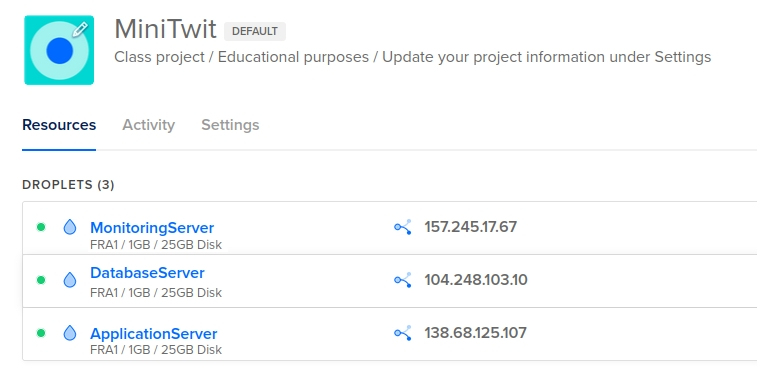
\includegraphics[scale=.5]{images/digitalocean_droplets.jpg}
    \caption{Caption}
    \label{fig:digitalocean_droplets}
\end{figure}

% Identify threat sources
\subsubsection{Identify threat sources}
\textbf{Minitwit Web Application Server} - A vulnerability assessment with tools was done, with several tools. The full report\cite{security_assesment_report} showed that we had several high risk threats. These threats include: 

\begin{enumerate}
    \item Path Traversal
    \item SQL Injection
    \item Absence of Anti-CSRF Tokens
    \item CSP Header Not Set
    \item Missing Anti-clickjacking Header
\end{enumerate}

A path traversal attack aims to gain access to directories and files, which are not stored in the web root folder\cite{owasp_path_traversal}. When running the automated vulnerability assessment, patch traversal was highlighted as a high risk threat. However, this does not seem to be relevant for our web-application, since it is impossible to access sensitive directories and files with "dot-dot-slash" sequences.


SQL injection attacks consists of injecting SQL queries through input fields in a web-application\cite{owasp_sql_injection}. This attack can be used to maliciously modify database columns or even execute administrator operations on the database itself. However, this is not an issue for our application, since we're using an object-relational-mapping (ORM) to handle all database operations. Thus, we're not using dynamic queries to execute operations on the database, but delegate this to the ORM. This means that the efficacy of any SQL injection attack depends on the integrity of the ORM that we're using for our MiniTwit application. In this case, we're using GORM.\cite{gorm}


Adding Anti-CSRF Tokens is also suggested by the vulnerability scanner. This makes sense, since this does not seem to be handled by default by Gin. In this case, it is worth to think about the impact an CSRF-attack would have on our MiniTwit application. A successful CSRF-attack is only limited to the privileges of the user and in this case, these include tweeting, following and unfollowing users.


Lastly it is important to note, that the application does not have any rate limiting. So it would be possible to deploy a \gls{dos} brute-force attack on the /login page, to obtain valid username and password combinations.

\textbf{Postgres Database Server}
The database server has several services running, with WAN exposed ports like the Postgres server through NGINX and the node exporter service, with only the postgres server really being of interest. This can be seen on \autoref{fig:database_system_diagram}

Threats to the postgres server could be if it was used to do privilege escalation on the machine that it is running on, which seems pretty unlikely. In a real business scenario data exfiltration could also be a threat, if any customer GDPR or business crucial data was present in the database. 

\begin{figure}[H]
    \centering
    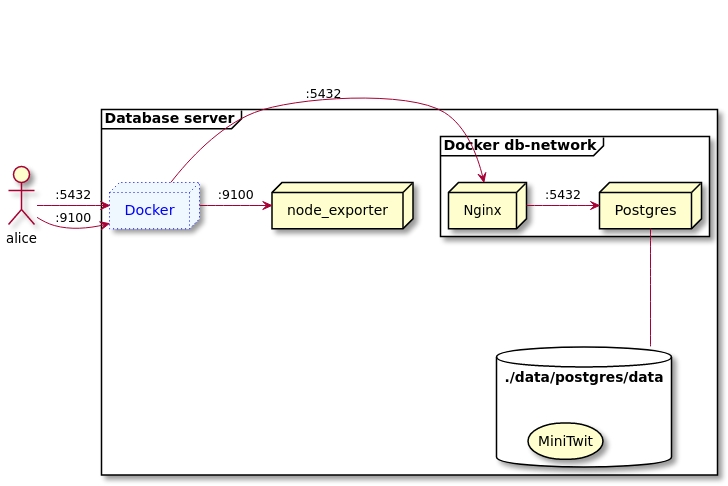
\includegraphics[scale=0.4]{images/diagrams/database/database.jpg}
    \caption{Database server diagram}
    \label{fig:database_system_diagram}
\end{figure}

\textbf{Logging and Monitoring Server}

The Logging and Monitoring server also has several services running, with WAN exposed ports through NGINX to: Loki, Grafana and Prometheus. Prometheus also talk to a node exporter and the groups own datascraper service. This can be seen on \autoref{fig:monitoring_logging_server}.
Loki is used to gather logging information from the application and Prometheus is gathering  infrastructure metrics for monitoring. 

Threats to these services:

\begin{enumerate}
    \item Access to the Grafana dashboard might reveal business or deployment sensitive information.
    \item Privilege escalation vulnerabilities to the machine in any of the service.
\end{enumerate}


\begin{figure}[H]
    \centering
    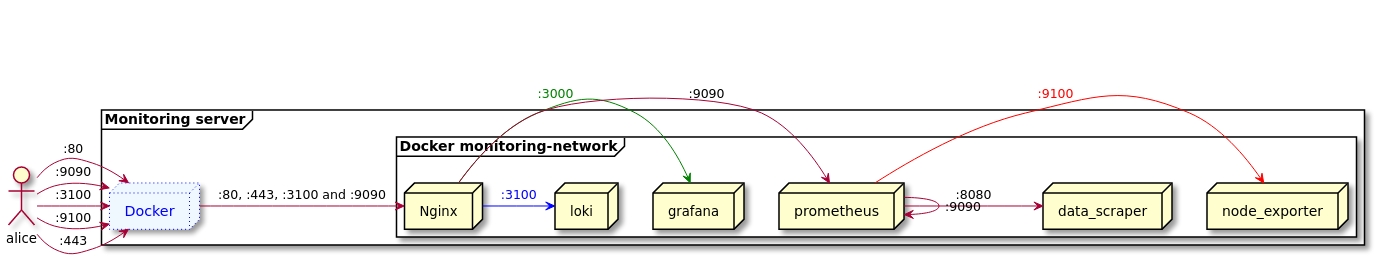
\includegraphics[scale=0.3]{images/logging/monitoring_logging.jpg}
    \caption{Monitoring and Logging server diagram}
    \label{fig:monitoring_logging_server}
\end{figure}

\textbf{DigitalOcean as Cloud Provider}
DigitalOcean is used by the group as the Cloud provider, which offers a website for teams to configure their cloud infrastructure. The configuration can also be accessed through a REST API with an API key, which can be used to provision and configure current or new VMs. The website also provides a "web console", which gives the authorised user a web terminal, with access to the root user of the VMs. 

\textbf{Github as Code Version Control, \acrshort{scm}, project documentation and CI/CD provider}
The group uses Github for both its version control and doing Continues Integration with Github Actions. Since all the code is in public repositories, the group has to be extra cautious whenever pushing and dealing with secrets in the codebase. Another point, which was mentioned by Helge was that it can be a bit of a risk to depend on a single service provider like Microsoft's Github for multiple functions/roles. 

\textbf{Discord Channel as secret sharing and communication} - Is the group's chosen method of communication and sharing secrets like Digital Ocean API keys, database passwords and etc. in cleartext. Discord is a communication platform, which is mostly used by the gaming community and thus not directly targeted to enterprise use. The platform has access control and with the use of a private server, should make it so it is for invited members only. However, scams\cite{discord_privacy} that lead to account takeovers or misconfigured server permissions, can lead to outsiders accessing "private" channels without being authorized and viewing secrets.


% Risk scenarios
\subsubsection{Risk scenarios, their impact and likelihood}

\textbf{Minitwit Web Application Server}
An adversary could in case of a SQL injection vulnerability get access to mess with the database server.(1) Not very likely, but could have high impact.

Another scenario would be that the response time of service would be degraded due to a password brute-force or a dedicated \gls{dos} attack.(2) Highly likely with medium impact, depending on the degree of degradation. 


\textbf{Postgres Database Server}
The current configuration of the server leaves the database open to anyone trying to brute-force access to the postgres database, which is only protected by a password.(3) Highly likely with high impact.


\textbf{Logging and Monitoring Server}
A successful bruteforce attack of the grafana login page could lead to people getting access to business data and possibly get information about the database server setup.(4) Not very likely with low impact.


\textbf{DigitalOcean as Cloud Provider}
The API key is leaked by a member through the Discord channel or in a commit to the public Github repository. The API key could then be used to destroy/remove the group's infrastructure. A worse scenario would be, that the intruder spins up powerful VM's (driving up our bill) and use them for cryptocurrency mining, connect them to a botnet or use them for criminal activity.(5) Not very likely with High impact.

Another scenario would be that one of the team members does not follow common password-policy practices, and therefore has the same passwords for several accounts with the same email address. Then in an event that there is a database/password-leak on any service that the member uses, an intruder could get access to all additional services like the member's DO account. By having access to the account the intruder could upload their own keys to the servers or simply use the web-based terminal to gain root access to the servers. (6) Not very likely with High impact.

\textbf{Github as Code Version Control, \acrshort{scm}, project documentation and CI/CD provider}
The group uses Github for both its version control and doing Continues Integration with Github Actions. Since all the code is in public repositories, the group has to be extra cautious whenever pushing and dealing with secrets in the codebase. (7) Highly likely, since the group has already tried it with medium-high impact.

Another point, which was mentioned by Helge was that it can be a bit of a risk to depend on a single service provider like Microsoft's Github for multiple functions/roles. 


\textbf{Discord Channel as secret sharing and communication}
Someone gets access to one of the developers account, who accidentally also uses their Discord account in their spare time.(8) Or access could be given through an invitation link, by adding a malicious Discord Bot or by using other social-engineering tricks. Not very likely with High impact.

\subsection{Risk Analysis}
% Use a Risk Matrix to prioritize risk of scenarios
% Discuss what are you going to do about each of the scenarios
From the previous section, the following risk matrix can be created.

\begin{table}[H]
\centering
\begin{tabular}{|l|
>{\columncolor[HTML]{34FF34}}l |
>{\columncolor[HTML]{F8FF00}}l |
>{\columncolor[HTML]{FE0000}}l |}
\hline
Likelihood/Impact & Low                      & Medium                      & High                          \\ \hline
Likely            & \cellcolor[HTML]{F8FF00} & \cellcolor[HTML]{FE0000}2,7 & 3                             \\ \hline
Possible          &                          &                             & 1                             \\ \hline
Unlikely          & 4                        & \cellcolor[HTML]{34FF34}    & \cellcolor[HTML]{F8FF00}5,6,8 \\ \hline
\end{tabular}
\end{table}

From this, we can sort the scenarios in a prioritised order: "3,2,7,1", where likelihood is more important than impact. The following mitigation plan based on discussion and research was decided on. 

\textbf{Postgres Database Server password bruteforce (3)}
Instead of having the postgres server open up for password-authentication, the team could setup an alternative authentication method like Kerberos, described in the postgres documentation\cite{postgres_auth_methods}.
Alternatively setting up SSH connection or simply setup a VPN between the application server and the database server.

\textbf{Minitwit Web Application Server DoS or bruteforce (2)}
Setup rate limiting in the post message and login endpoints, will result in it becoming harder to do those attacks. Anti DDos solutions like proxying traffic through Cloudflare or use a CDN for static content, are also popular mitigation strategies.\cite{owasp_dos_mitigation }

\textbf{Github as Code Version Control, \acrshort{scm}, project documentation and CI/CD provider (7)}

\textbf{Minitwit Web Application Server DoS or bruteforce (1)}